\documentclass[a4paper,12pt]{article}
\usepackage[top=2cm, bottom=2cm, left=2cm, right=2cm]{geometry}
\usepackage[french]{babel}
\usepackage[T1]{fontenc}
\usepackage[utf8]{inputenc}
\usepackage{hyperref}
\usepackage{graphicx}

\title{Catégorisation automatique de textes}
\author{Agathe \textsc{Mollé}}
\date{}

\begin{document}

	\maketitle

	\section*{Introduction}
		Nous nous intéressons à la tâche de catégorisation (classification) automatique de textes. Cette tâche consiste à employer de l'apprentissage supervisé afin de déterminer à quelle catégorie (classe) appartient un texte.

		Ce rapport présente une comparaison des principales méthodes de catégorisation, ainsi qu'une comparaison de sélection de caractéristiques.

	\section*{Corpus}
		Nous utilisons les données du corpus Reuters, comportant 10 788 documents, soit 1,3 millions de mots. Ces documents sont étiquetés selon 90 catégories, chaque document possédant en général plusieurs catégories. Le découpage des ensembles d'entraînement (70\%) et de test (30\%) est déjà effectué.

	\section*{Méthodes évaluées}
		Nous cherchons à comparer certaines méthodes de classification ainsi que des méthodes de sélection de caractéristiques.

		\paragraph*{Catégorisation}
			Nous nous intéressons aux méthodes de catégorisation suivantes :
			\begin{itemize}
				\item Classification naïve de Bayes (Multinomiale, Bernoulli)
				\item Séparateur à vaste marge (SVM)
				\item K plus proches voisins
				\item Algorithme de Rocchio
				\item Réseau de neurones : le perceptron
			\end{itemize}

		\paragraph*{Sélection de caractéristiques}
			En ce qui concerne la sélection de caractéristiques, nous testons deux méthodes :
			\begin{itemize}
				\item Fréquence de document pondérée (tf-idf)
				\item Manque d'indépendance entre un mot et une catégorie ($\chi^2$)
			\end{itemize}

	\section*{Implémentation}
		Les tests ont été effectués à l'aide d'un script python. Celui-ci utilise les bibliothèques nltk et sklearn. Pour exécuter le script, il suffit de lancer la commande :
		\begin{verbatim}
			python categ.py
		\end{verbatim}
		Le code est disponible sur \href{https://github.com/Ehtaga/document-categorization}{Github}.

	\section*{Mesures}
		Pour évaluer la pertinence des classifieurs, nous utilisons les mesures classiques d'apprentissage supervisé, à savoir la précision, le rappel ainsi que la F-mesure.

	\section*{Résultats}
		Voici les résultats obtenus pour les différents classifieurs étudiés :

		%\subsection*{Multinomial Naive Bayes}
		\begin{table}[h!]
			\centering
			\begin{tabular}{l|c c c}
				& Précision & Rappel & F-mesure\\
				\hline
				tf-idf & .42 & .53 & .47\\
				$\chi^2$ & .66 & .68 & .67\\
			\end{tabular}
			\caption{Multinomial Naive Bayes}
		\end{table}

		\begin{table}[h!]
			\centering
			\begin{tabular}{l|c c c}
				& Précision & Rappel & F-mesure\\
				\hline
				tf-idf & .46 & .56 & .50\\
				$\chi^2$ & .67 & .64 & .65\\
			\end{tabular}
			\caption{Bernoulli Naive Bayes}
		\end{table}

		\begin{table}[h!]
			\centering
			\begin{tabular}{l|c c c}
				& Précision & Rappel & F-mesure\\
				\hline
				tf-idf & .73 & .75 & .74\\
				$\chi^2$ & .70 & .71 & .71\\
			\end{tabular}
			\caption{SVM}
		\end{table}

		\begin{table}[h!]
			\centering
			\begin{tabular}{l|c c c}
				& Précision & Rappel & F-mesure\\
				\hline
				tf-idf & .67 & .69 & .68\\
				$\chi^2$ & .62 & .63 & .62\\
			\end{tabular}
			\caption{K plus proches voisins}
		\end{table}

		\begin{table}[h!]
			\centering
			\begin{tabular}{l|c c c}
				& Précision & Rappel & F-mesure\\
				\hline
				tf-idf & .71 & .69 & .70\\
				$\chi^2$ & .69 & .60 & .64\\
			\end{tabular}
			\caption{Algorithme de Rocchio}
		\end{table}

		\begin{table}[h!]
			\centering
			\begin{tabular}{l|c c c}
				& Précision & Rappel & F-mesure\\
				\hline
				tf-idf & .73 & .70 & .72\\
				$\chi^2$ & .66 & .64 & .65\\
			\end{tabular}
			\caption{Perceptron}
		\end{table}

		\begin{figure}[h!]
		\centering
		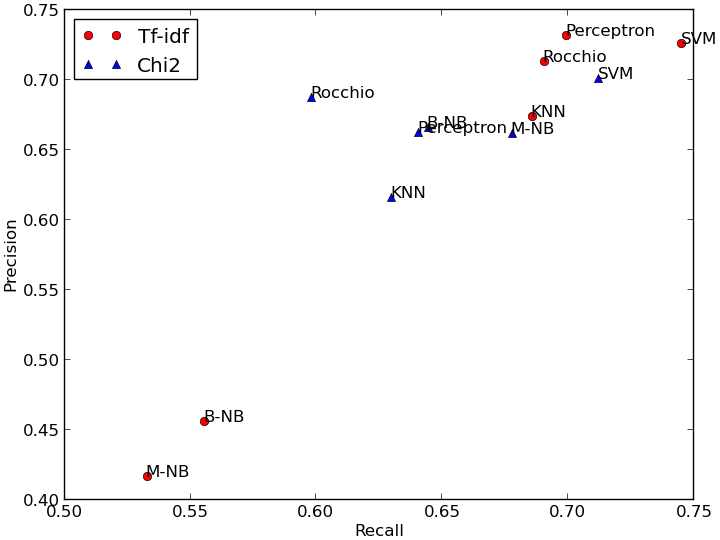
\includegraphics{graph.png}
		\caption{Comparaisons des différentes de méthodes de catégorisation}
		\end{figure}


	\section*{Discussion}

		Les classifieurs naïfs de Bayes sont moins efficaces lorsque les caractéristiques s'appuient sur la fréquence des mots dans le document. Ils sont cependant plus intéressants en utilisant la mesure $\chi^2$.

		De manière générale, la catégorisation naïve de Bayes et les K plus proches voisins obtiennent des résultats moins intéressants que la méthode des centroïdes, celle du Perceptron ainsi que SVM.

		Il aurait été intéressant d'étudier la catégorisation par arbres de décisions, mais nltk ne permet pas de les implémenter correctement, du moins nous n'avons pas su l'exploiter.

		En définitive, ces résultats permettent d'obtenir un aperçu des principales méthodes de catégorisation. Cependant, cette étude ne prend pas en compte la multiplicité des catégories attribuées à un même document. En effet, les mesures ne s'intéressent qu'à la classe la plus représentée. Il serait donc intéressant d'entraîner un classifieur par catégorie, soit 90 dans notre cas.

\end{document}